\section{Systemmodell}

\subsection{Schichtenübersicht}
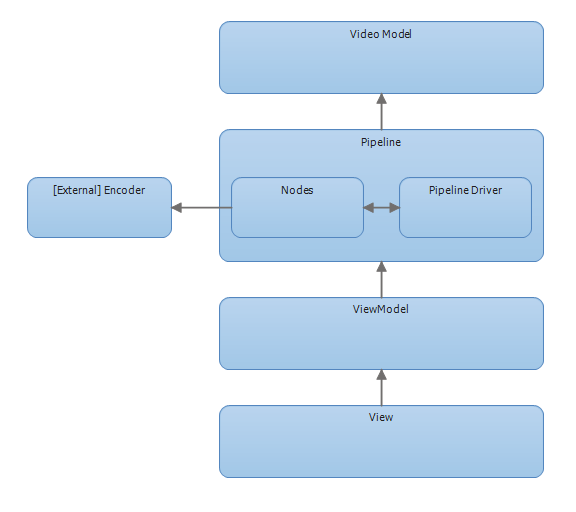
\includegraphics[scale=0.75]{resources/Layers}

\subsection{Schichtendetails}

\subsubsection*{Video Model}
Das Video Model repräsentiert ein eingelesenes Video, ggf. mit zugehörigen
Log-Daten. Da es die Daten im RGB-Format speichert, müssen diese bei Eingabe,
Ausgabe und Interaktion mit dem Encoder vom bzw. ins YUV-Format konvertiert
werden (siehe auch \hyperref[sec:produktdaten]{Produktdaten}).

\subsubsection*{Encoder}
Der zu testende Encoder ist eine externe Komponente, die nach Angabe ihres
Dateipfads vom entsprechenden Pipeline-Knoten angesprochen wird.

\newpage
\subsubsection*{Pipeline}
Die Pipeline-Schicht repräsentiert den UI-unabhängigen Aufbau des
Analyse-DAGs\footnote{\emph{directed acyclic graph}}. Sie besteht einerseits aus
den unterschiedlichen Knoten-Klassen, die unabhängig voneinander ihren
jeweiligen Algorithmus auf Frame-für-Frame-Basis implementieren, und
andererseits aus dem Pipeline Driver, der für die Abhängigkeitsauflösung und
letztendliche Abarbeitung der Pipeline zuständig ist.

\subsubsection*{ViewModel} Nach dem
Model-View-ViewModel-Pattern\footnote{\url{http://en.wikipedia.org/wiki/MVVM}}
(MVVM) ist es Aufgabe der ViewModel-Schicht, das Model der View in einer für sie
verarbeitbaren Form zu präsentieren. Bezogen auf das Projekt bedeutet dies vor
allem, die Model-Klassen um View-spezifische Daten (wie Positionierung auf der
Oberfläche) und Methoden zu ergänzen.

\subsubsection*{View}
Unter WPF wird die Oberfläche in der Beschreibungssprache
XAML\footnote{\url{http://msdn.microsoft.com/en-us/library/ms752059.aspx}}
erstellt. Sie steht über Datenbindung mit dem ViewModel in Verbindung und leitet
Benutzereingaben an dieses weiter, sodass sie selbst wenig Logik enthalten muss.
